%%%%%%%%%%%%%%%%%%%%%%%%%%%%%%%%%%%%%%%%%
% 
% LaTeX Template
% Version 3.1 (25/3/14)
%
%%%%%%%%%%%%%%%%%%%%%%%%%%%%%%%%%%%%%%%%%

%----------------------------------------------------------------------------------------
%	PACKAGES AND DOCUMENT CONFIGURATIONS
%----------------------------------------------------------------------------------------

\documentclass[12pt, a4 paper]{article}

\usepackage{hhline}
\usepackage{tikz}
%\usepackage[top=2cm, bottom=2cm, outer=0cm, inner=0cm]{geometry}
\usepackage{graphicx} % Required for the inclusion of images
\usepackage{multicol} % Required for multicolumns
\usepackage{setspace} % Required for line spacing
\setlength\parindent{0pt} % Removes all indentation from paragraphs
\setlength{\columnseprule}{0.4pt} % Adds vertical line between multicolumns
\usepackage{multirow} % Required for multirows
\usepackage{booktabs} % For prettier tables
\usepackage{xcolor}
%\usepackage{tabularx}
%\renewcommand{\rmdefault}{ptm}

%\usepackage{helvet}
\usepackage{ragged2e}
\usepackage{times} % Uncomment to use the Times New Roman font

%----------------------------------------------------------------------------------------
%	DOCUMENT INFORMATION
%----------------------------------------------------------------------------------------

\begin{document}

\tikz[remember picture,overlay] \node[inner sep=0pt] at (current page.center){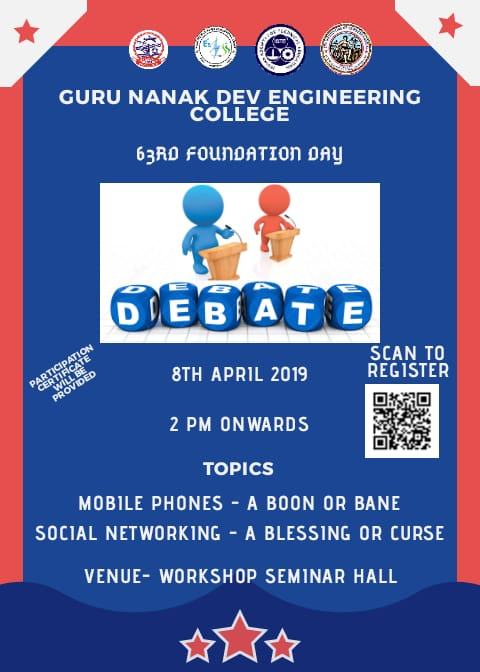
\includegraphics[width=\paperwidth,height=\paperheight]{image1.jpg}};

\clearpage

%\font\myfont=cmr12 at 35pt
%\title{\myfont  Event Name} % Write Event name here
%\author{}
%\date{\vspace{-10ex}}

%\maketitle % Insert the title, author and date
\setstretch{1.5}

\tikz[remember picture,overlay] \node[opacity=0.8,inner sep=0pt] at (current page.center){
\includegraphics[width=\paperwidth,height=\paperheight]{Border48-A4--Arvin61r58.png}};
%\tikz[remember picture,overlay] \node[opacity=0.5,inner sep=0pt] at (current page.center){\includegraphics[width=\paperwidth,height=\paperheight]{color-2174049__340.png}};

\begin{center}
\Huge \bfseries \ttfamily Debate
\end{center}

\begin{center}
\large An oratory-skill event
\end{center}

\begin{center}
\begin{multicols}{2}
\begin{tabular}{l r}
Date: & 08/04/2019\\ % Date the event was held
Time: & 2:00 P.M to 4:00 P.M \\ % Time of event 
\end{tabular}
\columnbreak
\begin{tabular}{l r}
Venue: & Workshop Seminar Hall \\ % Venue of event

\end{tabular}
\end{multicols}

\medskip
\justify
\begin{large}
\setstretch{1}

 An oratory-skill event, ‘DEBATE’ was organized by ISTE (India Society for Technical Education) in collaboration with SCIE and E2S2 on April 8,2019 in Workshop Seminar Hall. It was organized on the occasion of 63rd Foundation day of the institution.
 
\bigskip

\begin{multicols}{2}
The event was mainly organized to test the critical thinking skills of the students and their presentation of thoughts. The participants were judged on the basis of their content, presentation and organization of their debate.
\columnbreak

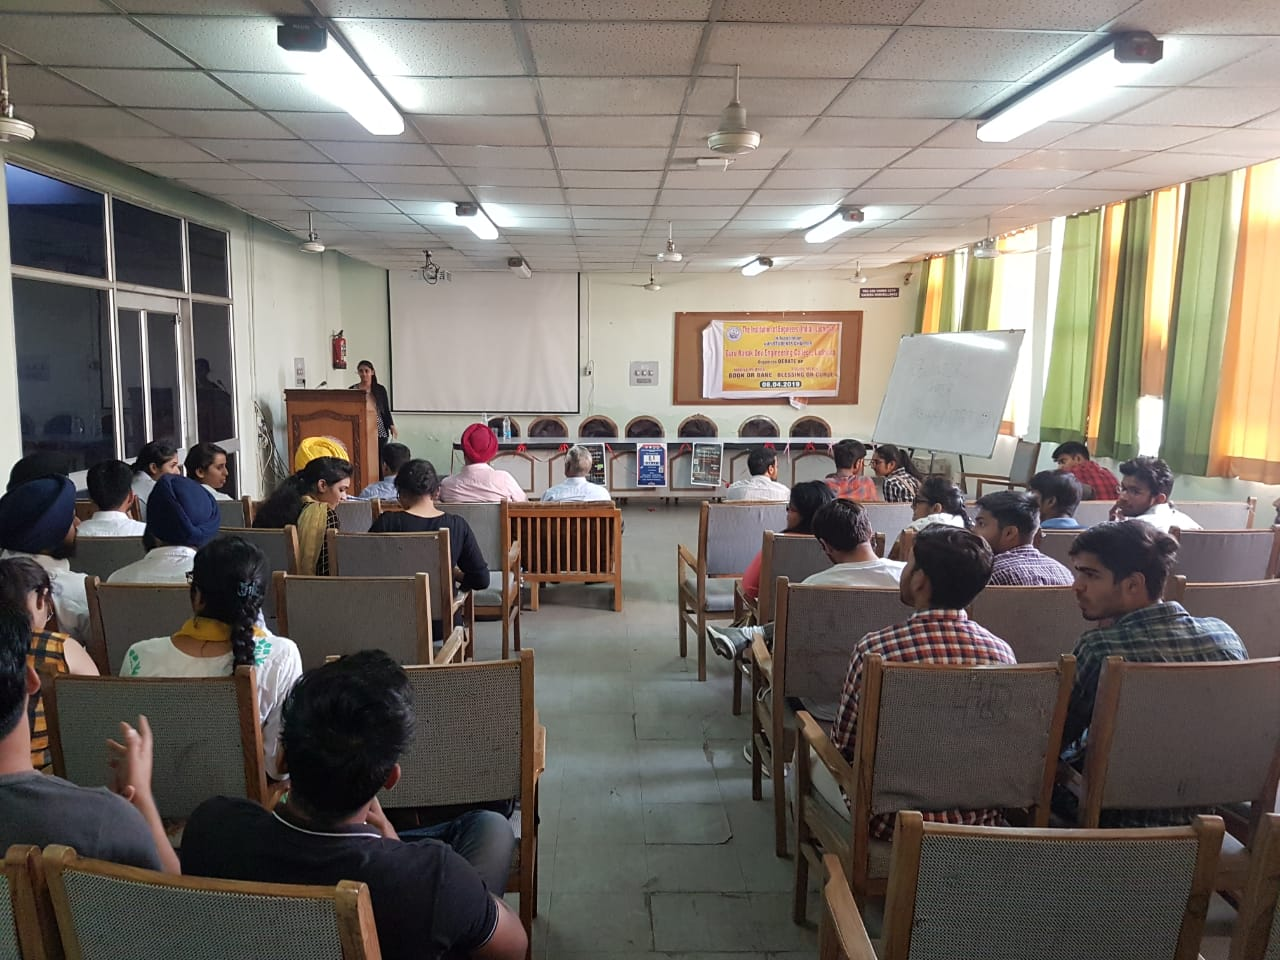
\includegraphics[width=\linewidth]{image6.jpg}
  
\end{multicols} 

The topics for the same were:-

\medskip
    1) Mobile Phones - A Boon or Bane

\medskip
    2) Social Networking - A Blessing or Curse
\newpage 

\tikz[remember picture,overlay] \node[opacity=0.8,inner sep=0pt] at (current page.center){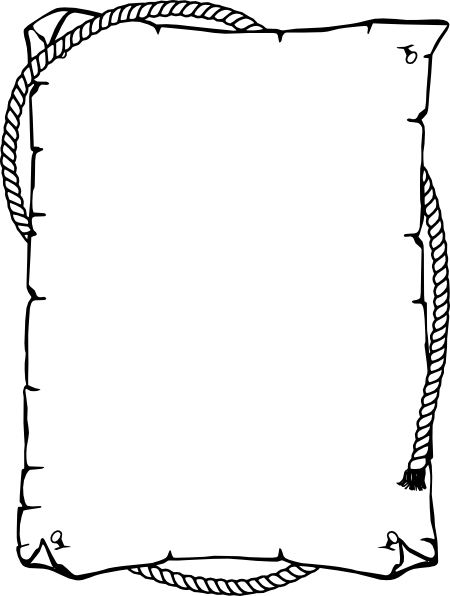
\includegraphics[width=\paperwidth,height=\paperheight]{5TRrp44jc.png}};

%\tikz[remember picture,overlay] \node[opacity=0.8,inner sep=0pt] at (current page.center){\includegraphics[width=\paperwidth,height=\paperheight]{md_5b0912b7c0870.png}};


The topics were disclosed 3 days prior to the event and the participants had to prepare either for the motion or against.

\bigskip
\begin{multicols}{2}
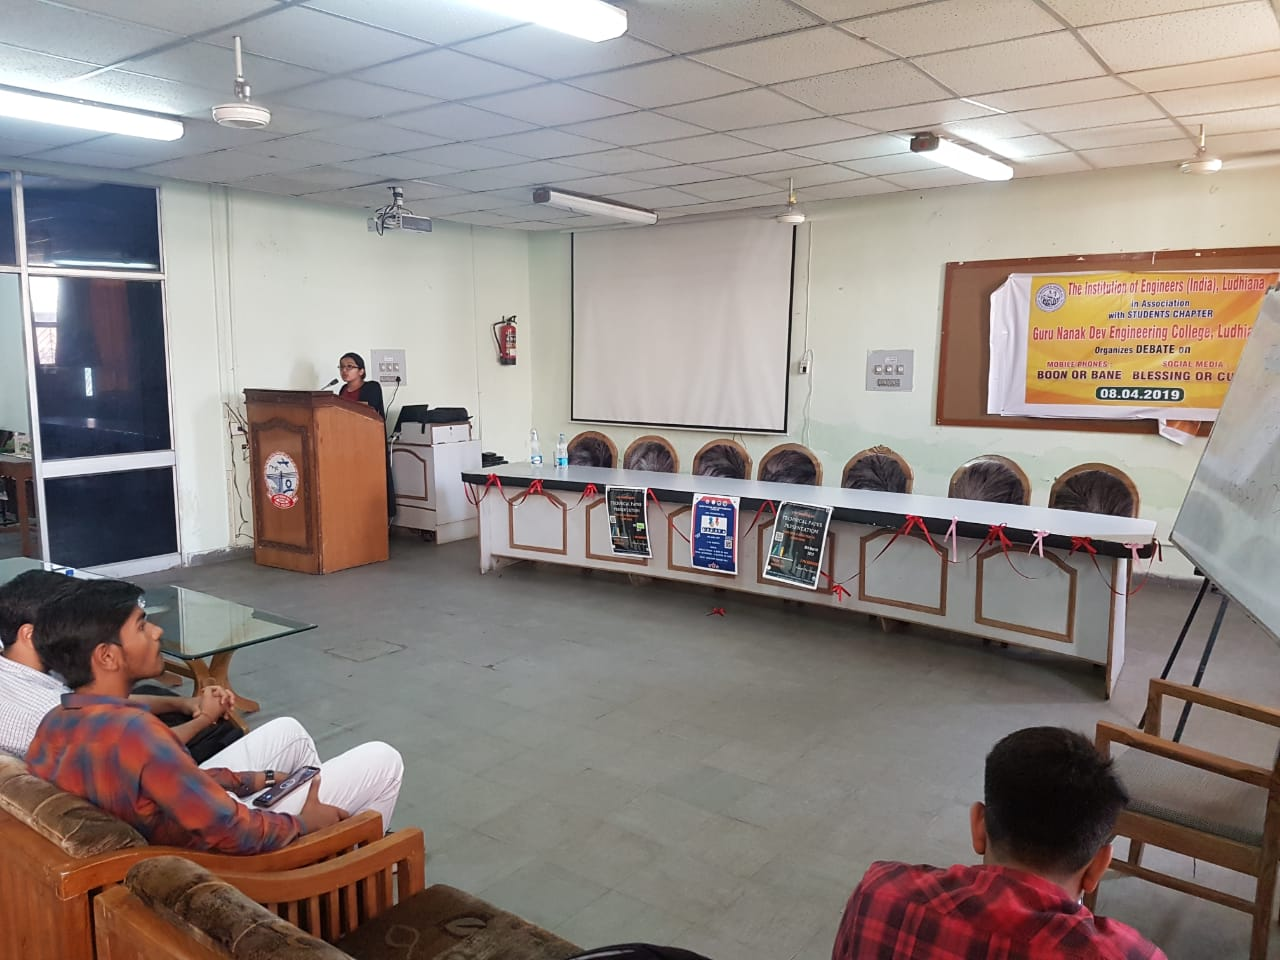
\includegraphics[width=\linewidth]{image5.jpg}

\columnbreak
\large Each participant was allotted a maximum time of 3 minutes. During the course of debate, First Bell rang at 3 minutes and he/she had to windup the speech within next 30 seconds after the second ring at 3:30 min nothing was taken into account from the speech.
  
\end{multicols} 
\bigskip

\bigskip
\begin{multicols}{2}
The usage of Written Material during speech delivery was prohibited and only cue reading was allowed . There was no language barrier , participants were given the freedom to speak in either one from Hindi, English or Punjabi.

\columnbreak
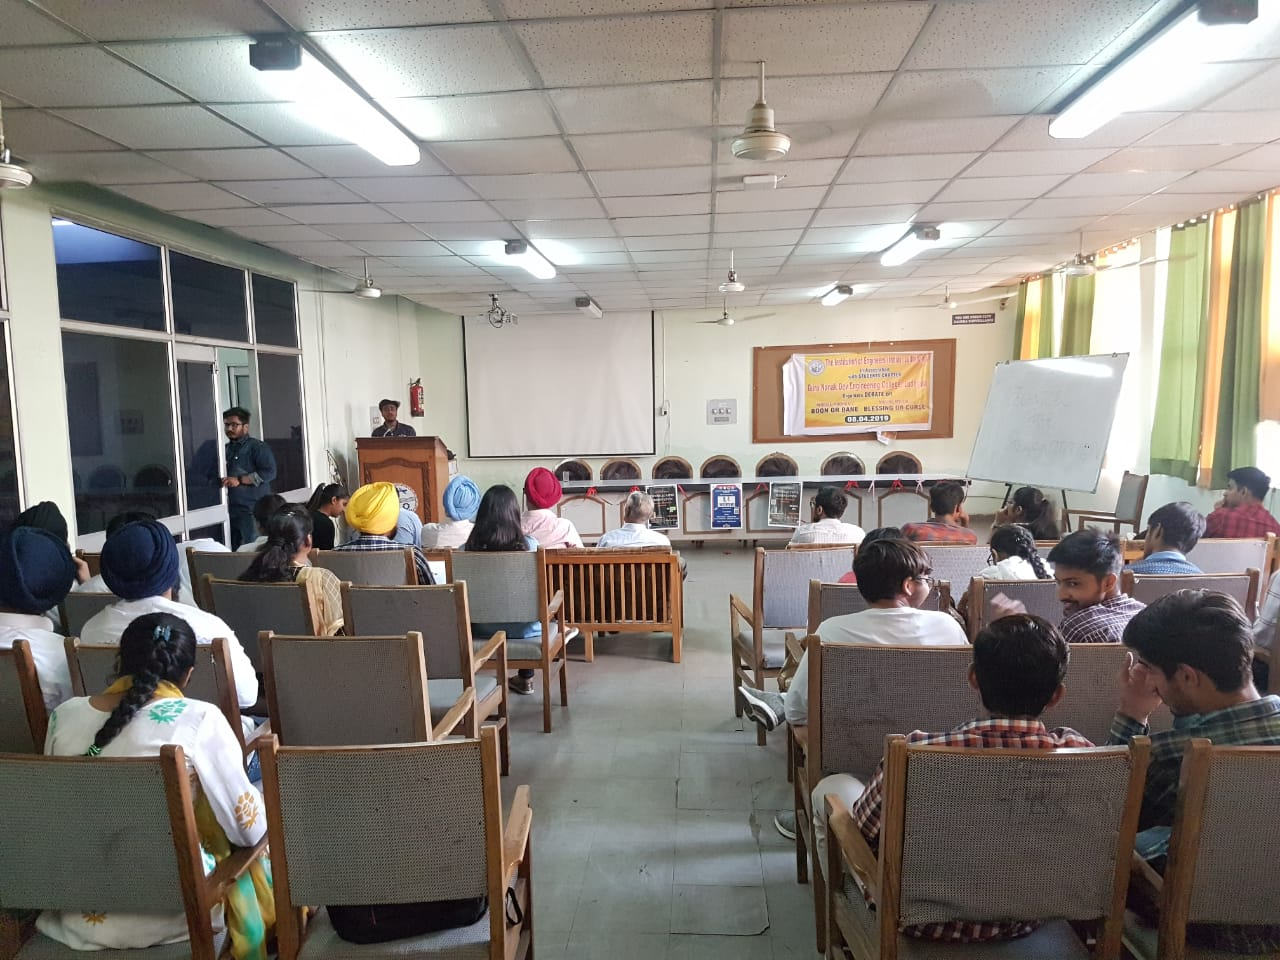
\includegraphics[width=\linewidth]{image2.jpg}

\end{multicols} 

\textbf{Judging Criteria :} 

Participants were judged on their :-

1)Content (Ideas, Logic and Effectiveness )

2)Presentation Style ( Delivery, Body Language)

3)Organization and Clarity ( Topic Development , Grammar , Pronunciation)
\end{large} 
\end{center}

\newpage 

\tikz[remember picture,overlay] \node[opacity=0.8, inner sep=0pt] at (current page.center){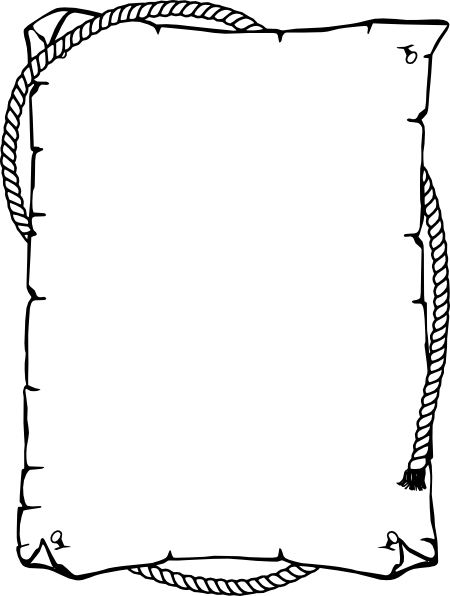
\includegraphics[width=\paperwidth,height=\paperheight]{5TRrp44jc.png}};
%\tikz[remember picture,overlay] \node[opacity=0.8,inner sep=0pt] at (current page.center){\includegraphics[width=\paperwidth,height=\paperheight]{md_5b0912b7c0870.png}};

\begin{center}
\Huge Glimpses of Event

\bigskip

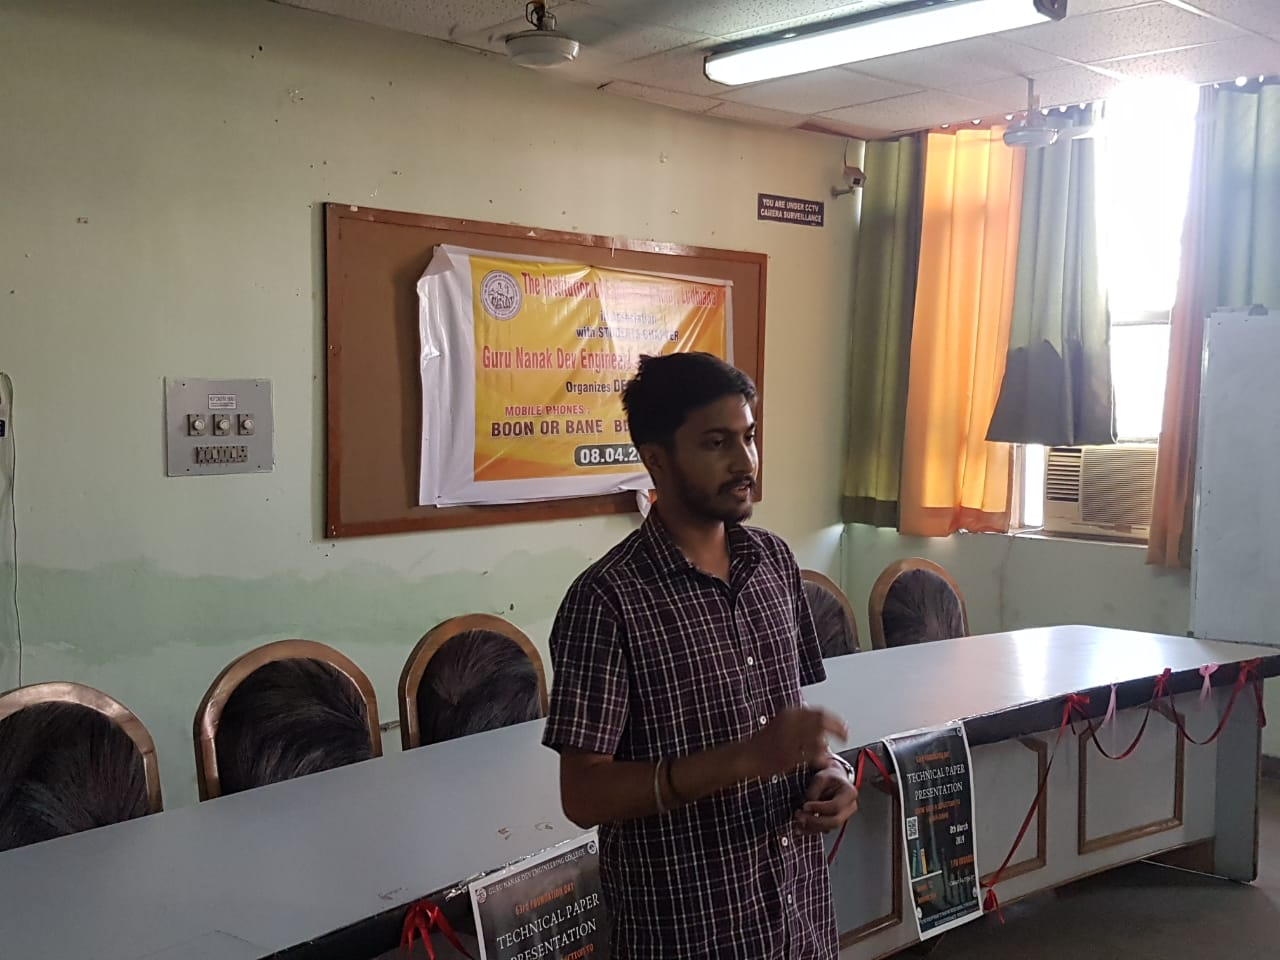
\includegraphics[height=7cm]{image4.jpg}

\bigskip

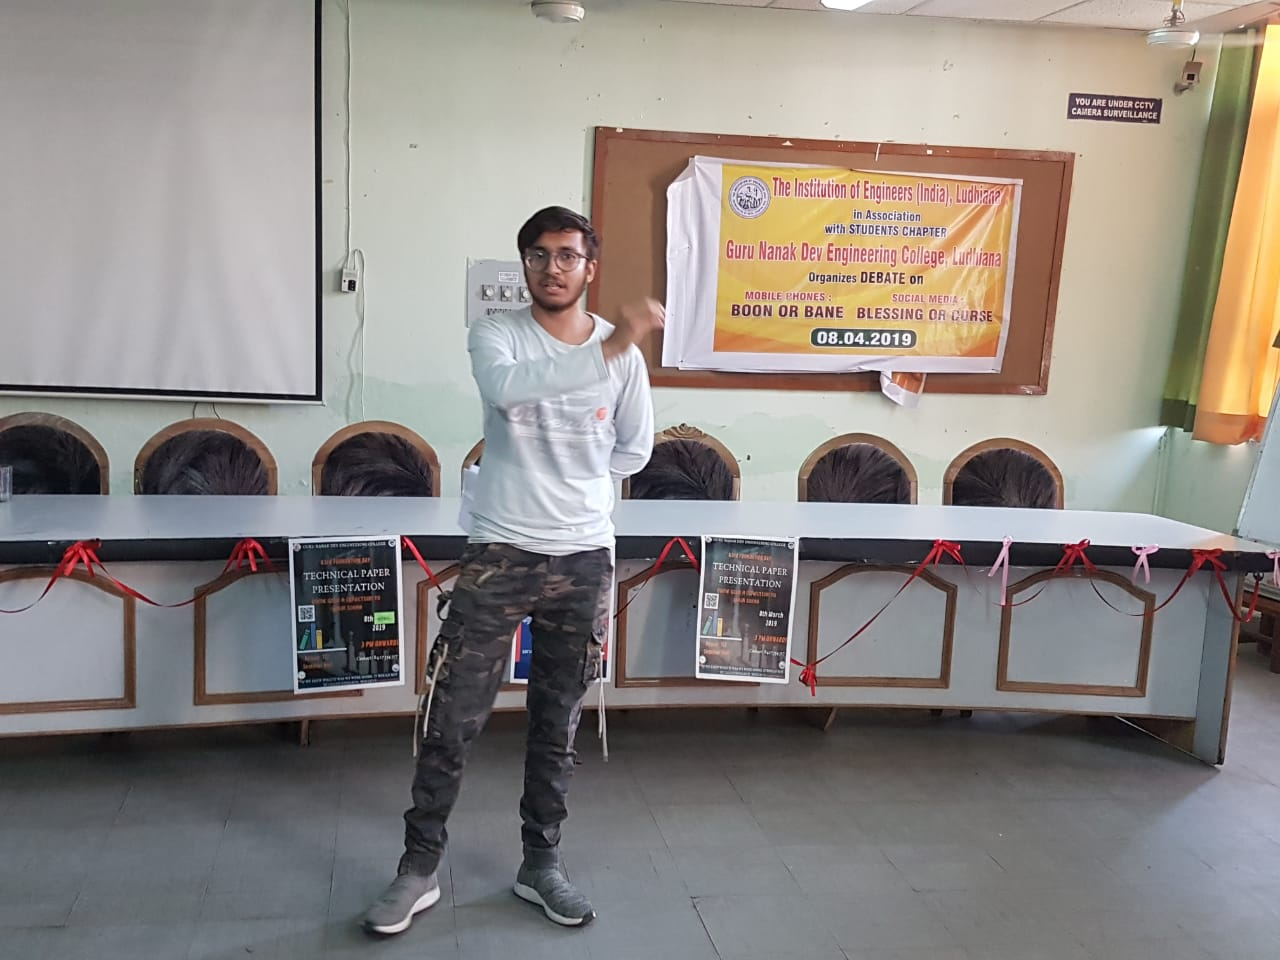
\includegraphics[ height=7cm]{image3.jpg}

\end{center}

\newpage

\tikz[remember picture,overlay] \node[opacity=0.8,inner sep=0pt] at (current page.center){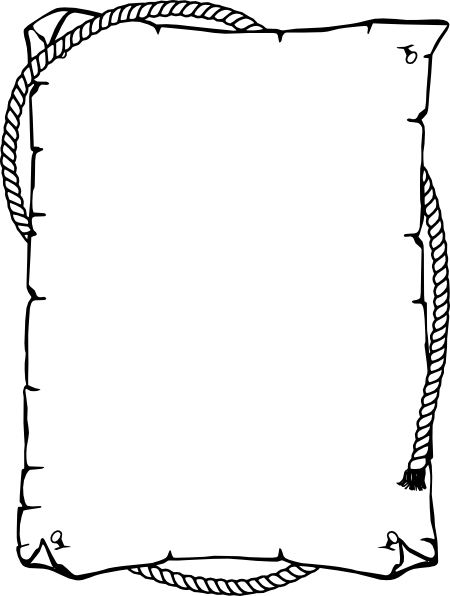
\includegraphics[width=\paperwidth,height=\paperheight]{5TRrp44jc.png}};

\begin{center}
\huge Organisers list
\end{center}

\begin{table}[h!]
                        \centering
\begin{tabular}{p{0.65in}p{2.66in}p{1.28in}p{0.96in}}
\hline
%row no:1
\multicolumn{1}{|p{0.65in}}{\Centering \textbf{S.NO.}} & 
\multicolumn{1}{|p{1.66in}}{\Centering \textbf{NAME}} & 
\multicolumn{1}{|p{1.28in}}{\Centering \textbf{YEAR/BRANCH}} & 
\multicolumn{1}{|p{0.96in}|}{\Centering \textbf{ROLL NO.}} \\
\hhline{----}
%row no:2
\multicolumn{1}{|p{0.65in}}{\Centering 1} & 
\multicolumn{1}{|p{1.66in}}{\Centering Darsbir Singh} & 
\multicolumn{1}{|p{1.28in}}{\Centering D3CSE} & 
\multicolumn{1}{|p{0.96in}|}{\Centering 1606667} \\
\hhline{----}
%row no:3
\multicolumn{1}{|p{0.65in}}{\Centering 2} & 
\multicolumn{1}{|p{1.66in}}{\Centering Karanjot Singh} & 
\multicolumn{1}{|p{1.28in}}{\Centering D3IT} & 
\multicolumn{1}{|p{0.96in}|}{\Centering 1607109} \\
\hhline{----}
%row no:4
\multicolumn{1}{|p{0.65in}}{\Centering 3} &
\multicolumn{1}{|p{1.66in}}{\Centering Arshdeep Kaur} &
\multicolumn{1}{|p{1.28in}}{\Centering D1CSE} &
\multicolumn{1}{|p{0.96in}|}{\Centering 1805161} \\
\hhline{----}
%row no:5
\multicolumn{1}{|p{0.65in}}{\Centering 4} &
\multicolumn{1}{|p{1.66in}}{\Centering Guneet Kohli} &
\multicolumn{1}{|p{1.28in}}{\Centering D1CSE} &
\multicolumn{1}{|p{0.96in}|}{\Centering 1805172} \\
\hhline{----}
%row no:6
\multicolumn{1}{|p{0.65in}}{\Centering 5} &
\multicolumn{1}{|p{1.66in}}{\Centering Sandeep} &
\multicolumn{1}{|p{1.28in}}{\Centering D2EE} &
\multicolumn{1}{|p{0.96in}|}{\Centering 1805365} \\
\hhline{----}
%row no:7
\multicolumn{1}{|p{0.65in}}{\Centering 6} &
\multicolumn{1}{|p{1.66in}}{\Centering Mayank Bakshi} &
\multicolumn{1}{|p{1.28in}}{\Centering D2EE} &
\multicolumn{1}{|p{0.96in}|}{\Centering 1819955} \\
\hhline{----}
%row no:8
\multicolumn{1}{|p{0.65in}}{\Centering 7} &
\multicolumn{1}{|p{1.66in}}{\Centering Ashutosh} &
\multicolumn{1}{|p{1.28in}}{\Centering D1CSE} &
\multicolumn{1}{|p{0.96in}|}{\Centering 1805165} \\
\hhline{----}
%row no:9
\multicolumn{1}{|p{0.65in}}{\Centering 8} &
\multicolumn{1}{|p{1.66in}}{\Centering Priyanka} &
\multicolumn{1}{|p{1.28in}}{\Centering D1EE} &
\multicolumn{1}{|p{0.96in}|}{\Centering 1805321} \\
\hhline{----}
%row no:10
\multicolumn{1}{|p{0.65in}}{\Centering 9} &
\multicolumn{1}{|p{1.66in}}{\Centering Divneet Kaur} &
\multicolumn{1}{|p{1.28in}}{\Centering D1CSE} &
\multicolumn{1}{|p{0.96in}|}{\Centering 1805169} \\
\hhline{----}

\end{tabular}
 \end{table}



\begin{center}
\huge Winners list
\end{center}

\begin{table}[h!]
                        \centering
\begin{tabular}{p{0.8in}p{2.73in}p{1.31in}p{0.86in}}
\hline
%row no:1
\multicolumn{1}{|p{0.8in}}{\Centering \textbf{S.NO.}} &
\multicolumn{1}{|p{1.73in}}{\Centering \textbf{NAME}} &
\multicolumn{1}{|p{1.31in}}{\Centering \textbf{YEAR/BRANCH}} &
\multicolumn{1}{|p{0.86in}|}{\Centering \textbf{ROLL NO.}} \\
\hhline{----}
%row no:2
\multicolumn{1}{|p{0.8in}}{\Centering 1} &
\multicolumn{1}{|p{1.73in}}{\Centering Maanvi Sharma} &
\multicolumn{1}{|p{1.31in}}{\Centering D3EE} &
\multicolumn{1}{|p{0.86in}|}{\Centering 1706690} \\
\hhline{----}
%row no:3
\multicolumn{1}{|p{0.8in}}{\Centering 2} &
\multicolumn{1}{|p{1.73in}}{\Centering Harnoor Singh} &
\multicolumn{1}{|p{1.31in}}{\Centering D1ECE} &
\multicolumn{1}{|p{0.86in}|}{\Centering 1805402} \\
\hhline{----}
%row no:4
\multicolumn{1}{|p{0.8in}}{\Centering 3} &
\multicolumn{1}{|p{1.73in}}{\Centering Achintya Tripathi} &
\multicolumn{1}{|p{1.31in}}{\Centering D2CSE} &
\multicolumn{1}{|p{0.86in}|}{\Centering 1706390} \\
\hhline{----}

\end{tabular}
 \end{table}

\newpage

\tikz[remember picture,overlay] \node[opacity=0.8,inner sep=0pt] at (current page.center){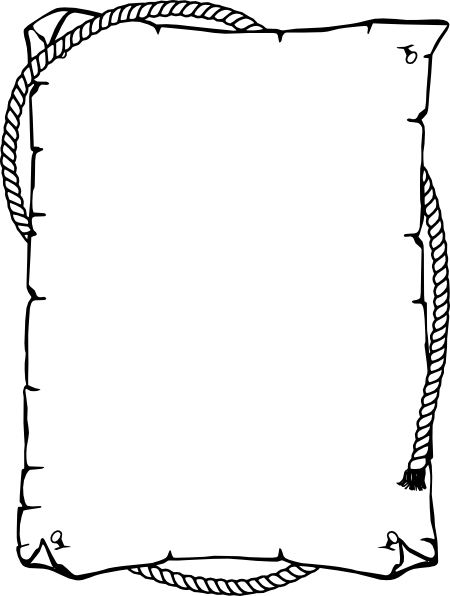
\includegraphics[width=\paperwidth,height=\paperheight]{5TRrp44jc.png}};
%\tikz[remember picture,overlay] \node[opacity=0.8,inner sep=0pt] at (current page.center){\includegraphics[width=\paperwidth,height=\paperheight]{md_5b0912b7c0870.png}};

\begin{center}
\huge Participants list
\end{center}

\begin{table}[h!]
  \begin{center}
    \begin{tabular}{|c|c|c|c|c|c|} 
    \toprule % <-- Toprule here
      \textbf{S.No.} & \textbf{Name} & \textbf{Branch} & \textbf{Year} & \textbf{URN}\\
      \midrule % <-- Midrule here
1       &Manpreet Kaur  &CSE    &1st    &1805200\\
2       &Simranjeet Kaur        &CSE    &1st    &1805992\\
3       &Harnoor Singh  &ECE    &1st    &1805402\\
4       &Ishpreet Kaur Gulati   &CSE    &2nd    &1706443\\
5       &Kamya Arora    &CSE    &2nd    &1706453\\
6       &Alpana &CE     &2nd    &1805126\\
7       &Achintya Tripathi      &CSE    &2nd    &1706390\\
8       &Kashish Nagori         &CE     &2nd    &1706231\\
9       &Shiv Shankar Kumar     &ECE    &3rd    &1607025\\
10      &Rampunit Kumar         &CE     &3rd    &1606536\\
11      &Maanvi Sharma  &EE     &3rd    &1706690\\
 \bottomrule % <-- Bottomrule here
    \end{tabular}
  \end{center}
\end{table}


\end{document}